\section{Theorie}
\label{sec:Theorie}

\subsection{Schwingungsgleichungen für kapazitiv gekoppelte Schwingkreise}

Obwohl im Folgenden ein elektromagnetischer Schwingkreis betrachtet wird, lassen sich die Erkenntnisse leicht auf ein mechanisches Analogon übertragen
(zum Beispiel ein gekoppeltes Schwingungssystem, bestehend aus 2 Fadenpendeln, die über eine elastische Feder miteinander verbunden sind 
\cite{Versuchsanleitung}). Der Grund, dass am elektrischen Schwingkreis Untersuchungen vorgenommen werden, ist, dass die Amplitude und die Frequenz
einfacher und genauer bestimmt werden können.
\newline
Mit Hilfe der Kirchhoffschen Knotenregel lässt sich für den Verzweigungspunkt A die Beziehung
\begin{equation}
    I_\text{k} = I_1 - I_2
    \label{eqn:Knotenregel}
\end{equation}
aufstellen.
\newline
Die Kirchhoffsche Maschenregel liefert zusätzlich jeweils für die beiden Leiterkreise 1 und 2 die Beziehung
\begin{equation}
    U_\text{C} + U_{\text{L}} + U_{\text{k}} = 0
    \label{eqn:Maschenregel}
\end{equation}
Außerdem gilt
\begin{equation}
    U_\text{C} = \frac{1}{C} \int I \, \symup{d}t
\end{equation}
  und
\begin{equation}
    U_\text{L} = L \dot{I}
\end{equation}
%Setzt man diese Beziehung in \ref {eqn:Knotenregel} ein erhält man 
%\begin{equation}
%    \frac{1}{C} \int I_1 \, \symup{d}t + L \dot{I_1} + \frac{1}{C_k} \int I_1 - I_2 \, \symup{d}t = 0
%\end{equation}
%und
%\begin{equation}
%    \frac{1}{C} \int I_2 \, \symup{d}t + L \dot{I_2} - \frac{1}{C_k} \int I_1 - I_2 \, \symup{d}t = 0
%\end{equation}
%Wenn man diese Gleichungen nun ein mal nach der Zeit differenziert und anschließend addiert \ref {eqn:Sieben} und subtrahiert \ref {eqn:Acht} erhält man
Es ergeben sich daraus Differentialgleichungen der Form
\begin{equation}
    L \frac{d^2}{dt^2}(I_1 + I_2) + \frac{1}{C}(I_1 +I_2) = 0
    \label{eqn:Sieben}
\end{equation}
und
\begin{equation}
    L \frac{d^2}{dt^2}(I_1 - I_2) + ( \frac{1}{C} + \frac{2}{C_{\text{K}}} ) (I_1 - I_2) = 0
    \label{eqn:Acht}
\end{equation}
%Damit hat man zwei unabhänig voneinader lösbare Differentialgleichungen, die als neue Variablen die Summe und Differenz der Ströme $ I_1 $ und $ I_2 $ haben.
%Aus den Lösungen der Differentialgleichungen \ref {eqn:Sieben} und \ref {eqn:Acht} ergeben sich die Frequenzen
Aus den Lösungen dieser Differentialgleichungen folgen die Frequenzen
\begin{equation}
    v^{+} = \frac{1}{ 2\symup{\pi} \sqrt{L C}}
    \label{eqn:Neun}
\end{equation}
und
\begin{equation}
    v^{-} = \frac{1}{ 2\symup{\pi} \sqrt{L (\frac{1}{C} + \frac{1}{C_{\text{K}}})^{-1}}}
    \label{eqn:Zehn}
\end{equation}
\newline
Werden nun zwei Spezialfälle des Systems der gekoppelten Oszillatoren betrachtet, so wird die Bedeutung der Frequenzen (\ref {eqn:Neun}) und (\ref {eqn:Zehn}) deutlich.
\newline
Wird angenommen, dass die Oszillation in beiden Schwingkreisen mit gleicher Amplitude und in Phase beginnt, also $ I_1 = I_2 $ gilt, dann wird die Differenzschwingung $ v^{-} $ (\ref {eqn:Zehn})
Null und beide Oszillatoren schwingen gleichphasig mit der Frequenz $ v^{+} $ (\ref {eqn:Neun}), die der des Einzeloszillators entspricht. Da sich die Ströme $ I_1 $ und $ I_2 $ konsequent
aufheben, liegt hierbei zu keinem Zeitpunkt Spannung am Kondensator $ C_{\text{K}} $ an.
\newline
Im zweiten Spezialfall wird angenommen, dass die Oszillatoren wieder mit gleicher Amplitude, jedoch entgegengesetzter Phase ($ I_1 = -I_2 $) beginnen zu schwingen. In diesem Fall
wird die Summenschwingung $ v^{+} $ \ref {eqn:Neun} Null und die beiden Oszillatoren schwingen gegenphasig mit der höheren Frequenz $ v^{-} $.
\newline
Diese beiden Spezialfälle und die zugehörigen Frequenzen werden als Fundamentalschwingungen bezeichnet.
\newline
Wird das System der gekoppelten Oszillatoren so angeregt, dass nur ein Oszillator zu Beginn eine von Null verschiedene Amplitude besitzt, so ergeben sich vollkommen andere Ergebnisse.
\newline
Werden die Lösungen der Differentialgleichungen (\ref {eqn:Sieben}) und (\ref {eqn:Acht}) zusammenaddiert und unter den gennanten
Anfangsbedingungen $ I_1 = 0 $ und $ I_2 \neq 0 $ betrachtet, ergibt sich daraus
\begin{equation}
    I_1(t) = \frac{1}{2} I_{1_0} (\cos v^{+} t + \cos v^{-} t )
    \label{eqn:Elf}
\end{equation}
und
\begin{equation}
    I_2(t) = \frac{1}{2} I_{1_0} (\cos v^{+} t - \cos v^{-} t )
    \label{eqn:Zwoelf}
\end{equation}
Mit Hilfe von Additionstheoremen können (\ref {eqn:Elf}) und (\ref {eqn:Zwoelf}) umgeschrieben werden zu
\begin{equation}
    I_1(t) = I_{1_0} \cos \frac{1}{2} (v^{+} + v^{-}) t \cos \frac{1}{2} (v^{+} - v^{-}) t
    \label{eqn:Dreizehn}
\end{equation}
und
\begin{equation}
    I_2(t) = I_{1_0} \cos \frac{1}{2} (v^{+} + v^{-}) t \cos \frac{1}{2} (v^{+} - v^{-}) t
    \label{eqn:Vierzehn}
\end{equation}
\newline
An (\ref {eqn:Dreizehn}) und (\ref {eqn:Vierzehn}) kann abgelesen werden, dass das System nun mit einer Frequenz von $ \frac{1}{2} (v^{+} + v^{-}) $ oszilliert.
Für diese Art von Oszillationen, die man Schwebungen nennt, wird angenommen, dass sich die Frequenzen $ v^{+} $ und $ v^{-} $ nur gering voneinander unterscheiden.
Demnach sind die Frequenz $ \frac{1}{2} (v^{+} + v^{-}) $ und die Frequenz des Einzeloszillators $ v^{+} $ ungefähr gleich.
\newline
Ebenso kann an (\ref {eqn:Dreizehn}) und (\ref {eqn:Vierzehn}) abgelesen werden, dass die Amplitude mit der Frequenz $ v^{-} - v^{+} $ zwischen Null und $ I_{1_0} $ oszilliert.
Diese Frequenz wird Schwebungsfrequenz genannt.

\subsection{Berechnung des Stromes in Abhängigkeit der Frequenz}


\begin{figure}[H]
    \centering
    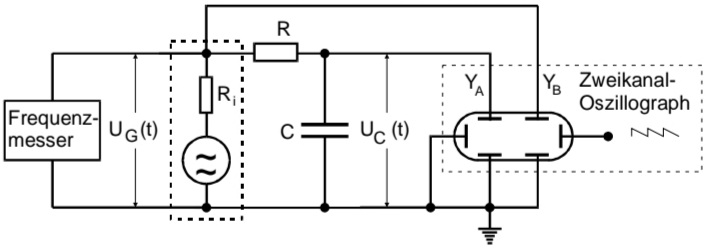
\includegraphics[width=0.75\textwidth]{plots/Schaltung3.png}
    \caption{Schaltbild für gekoppelte Schwingkreise \cite{Versuchsanleitung}}
    \label{fig:schaltung3}
\end{figure}

Wird der in \autoref{fig:schaltung3} dargestellte Schwingkreis durch eine Sinusspannung zu einer erzwungenen Schwingung angeregt
so folgt durch die Kirchhoffsche Maschenregel,
%Habe statt Bild einzufügen ein Zitat eingefügt und damit auf Anhang verwiesen

%ABBILDUNG 4 EINFÜGEN

%ABBILDUNG 4 EINFÜGEN

%ABBILDUNG 4 EINFÜGEN



\begin{equation}
    U = I_1 (z_C + z_L + z_{C_K} + z_R) - z_{C_K} I_2
    \label{eqn:Fuenfzehn}
\end{equation}
und
\begin{equation}
    0 = I_2 (z_C + z_L + z_{C_K} + z_R) - z_{C_K} I_1
    \label{eqn:Sechzehn}
\end{equation}
mit
\begin{center}
    $z_C = -j \frac{1}{wC}$,$z_L = jwL$, $z_{C_K} = -j \frac{1}{wC_K}$  und  $z_C = R$
\end{center}
%Für $I_2$ folgt nach Elimination von $I_1$
%\begin{equation}
%    I_2 = U \frac{-j\frac{1}{wC_k}}{(jwL - j(\frac{1}{wc} + \frac{1}{wC_k})+R)^2 + \frac{1}{w^2 {C_k}^2}}
%    \label{eqn:Siebzehn}
%\end{equation}
%\begin{equation}
%    \implies I_2 = U \frac{ -2wC_kRZ(w) + j(- \frac{1}{wC_k} + wC_kZ^2(w) - wR^2C_k) }{ 4w^2C_k^2R^2Z^2(w) + ( \frac{1}{wC_k} - wC_kZ^2(w) + wR^2C_k )^2 }
%    \label{eqn:Achtzehn}
%\end{equation} 
%mit
%\begin{equation}
%    Z(w) \coloneq wL - \frac{1}{w} (\frac{1}{C} + \frac{1}{C_k})
%    \label{eqn:Neunzehn}
%\end{equation}
Für den Betrag des Stromes gilt dann
\begin{equation}
    \lvert I_2\rvert = \lvert U\rvert \frac{1}{ 4w^2C_k^2R^2Z^2(w) + ( \frac{1}{wC_k} - wC_kZ^2(w) + wR^2C_k )^2 }.
    \label{eqn:Zwanzig}
\end{equation}
Bei den Fundamentalfrequenzen erreicht der Strom seine Maxima
\begin{equation}
    \lvert I(w^{+})\rvert = \frac{1}{ R\sqrt{4 + \frac{R^2C_k^2}{LC}}}
    \label{eqn:Einundzwandzig}
\end{equation}
und
\begin{equation}
    \lvert I(w^{-})\rvert = \frac{1}{ R\sqrt{4 + \frac{R^2C_k^2}{LC}(1+\frac{C}{C_k})}}.
    \label{eqn:Zweiundzwandzig}
\end{equation}
Diese Maxima können durch 
\begin{equation}
    \lvert I(w^{+})\rvert \approx \lvert I(w^{-})\rvert \approx \frac{1}{2R}
    \label{eqn:Dreiundzwandzig}
\end{equation}
genähert werden.


% \\ braucht man anscheinend garnicht, weil das Dokument, soweit ich erkennen kann, auch so gut formatiert ist